
 \documentclass[25pt, a0paper, portrait, margin=0mm, innermargin=15mm,
     blockverticalspace=15mm, colspace=15mm, subcolspace=8mm]{tikzposter} %Default values for poster format options.
     
\usepackage{tabularx,booktabs,adjustbox} % For tables
\usepackage{wrapfig,anyfontsize,lipsum}
\linespread{1.2}
\usetikzlibrary{calc,fit,arrows,decorations.pathmorphing,backgrounds,fit,positioning}
\usetikzlibrary{shapes.symbols}

\usepackage{color,colortbl}
\definecolor{Cblack}{rgb}{0,0,0}
\definecolor{Corange}{rgb}{0.9,0.6,0}
\definecolor{Cskyblue}{rgb}{0.35,0.7,0.9}
\definecolor{Cbluegreen}{rgb}{0,0.6,0.5}
\definecolor{Cyellow}{rgb}{0.95,0.9,0.25}
\definecolor{Cblue}{rgb}{0,0.45,0.7}
\definecolor{Cvermillion}{rgb}{0.8,0.4,0}
\definecolor{Cpurple}{rgb}{0.8,0.6,0.7}

\newcommand{\Cblack}[1]{\textcolor{Cblack}{#1}}
\newcommand{\Corange}[1]{\textcolor{Corange}{#1}}
\newcommand{\Cskyblue}[1]{\textcolor{Cskyblue}{#1}}
\newcommand{\Cbluegreen}[1]{\textcolor{Cbluegreen}{#1}}
\newcommand{\Cyellow}[1]{\textcolor{Cyellow}{#1}}
\newcommand{\Cblue}[1]{\textcolor{Cblue}{#1}}
\newcommand{\Cvermillion}[1]{\textcolor{Cvermillion}{#1}}
\newcommand{\Cpurple}[1]{\textcolor{Cpurple}{#1}}

 \newcommand{\magenta}[1]{\textcolor{magenta}{#1}}
 \newcommand{\teal}[1]{\textcolor{teal}{#1}}
  \newcommand{\gray}[1]{\textcolor{gray}{#1}}

% tikz colour settings
\tikzset{pop0/.style={red!50!yellow},pop1/.style={violet!80},pop2/.style={olive!70!green}}

\definecolorpalette{myColorPalette} {
\definecolor{colorOne}{named}{teal}
\definecolor{colorTwo}{named}{white}
\definecolor{colorThree}{named}{cyan}
}

 \tikzposterlatexaffectionproofoff %shows small comment on how the poster was made at bottom of poster

 % Commands
 \newcommand{\bs}{\textbackslash}   % backslash
 \newcommand{\cmd}[1]{{\bf \color{red}#1}}   % highlights command
% \newcommand{\crossmark}{\ding{55}}

 % Title, Author, Institute
 \title{{\bf Efficient simulation of identity-by-descent and ancestry in large datasets}}
 \author{{\bf Georgia Tsambos}}
 \institute{{\bf University of Melbourne, Australia}}

 % -- PREDEFINED THEMES ---------------------- %
 % Choose LAYOUT:  Default, Basic, Rays, Simple, Envelope, Wave, Board, Autumn, Desert,
 \usetheme{Autumn}
\usecolorstyle[colorPalette=myColorPalette]{Denmark}


 \begin{document}

     \maketitle
\block[bodyverticalshift=-2cm]{}{
   {\large\teal{
 Georgia Tsambos (1, 2), Peter Ralph (3), Jerome Kelleher (4), Stephen Leslie (1, 2, 5), Damjan Vukcevic (1, 2).
(1) School of Mathematics and Statistics, University of Melbourne, Australia (2) Melbourne Integrative Genomics, University of Melbourne, Australia, (3) Department of Mathematics, University of Oregon, United States, (4) Big Data Institute, University of Oxford, United Kingdom, (5) School of Biosciences, University of Melbourne, Australia.\\[7mm]
Presenting author: gtsambos (at) student.unimelb.edu.au}
}
}
   
   %%% BLOCK 0  
 \block[titleoffsety=1cm,bodyverticalshift=-20cm]{0. Introduction}{
 }
 \begin{columns}
 \begin{subcolumns}
   \subcolumn{31} \block[bodyoffsetx=1.5cm,bodyverticalshift=-5cm]{}{
{\fontsize{34}{35}\selectfont To assess the performance of methods in population genetics, we often wish to simulate realistic genetic datasets while retaining detailed information about the history of the simulated genomes.
This poster briefly describes how we can efficiently simulate genetic information with full information about the common ancestry of particular genomic segments, as well as information about the populations that these segments have been inherited from.
Although the software is still under development in \texttt{tskit} [1], our progress to date suggests that our methods are scaleable and fast enough to be useful in high-powered studies of subtle demographic questions.}\\[3mm] 
    }
 \end{subcolumns}
 \end{columns}

%%% BLOCK 1
     \begin{columns}%blocks will be placed into columns
         \column{.5}
         \block[roundedcorners=40,titleoffsety=-3cm,bodyoffsety=-3cm,bodyverticalshift=-1cm]{1. The data structure: tree sequences}{
\begin{center}
{\tt\small
\ldots GTAACGCGATAAGA\Cskyblue{T}ATTAGCCCAAAAACACAGACATGG\Cvermillion{A}AATAGCGTA\ldots \\
\ldots GTAACGCGATAAGA\Cvermillion{G}ATTAGCCCAAAAACACAGACATGG\Cskyblue{T}AATAGCGTA\ldots \\
\ldots GTAACGCGATAAGA\Cskyblue{T}ATTAGCCCAAAAACACAGACATGG\Cskyblue{T}AATAGCGTA\ldots \\
\ldots GTAACGCGATAAGA\Cvermillion{G}ATTAGCCCAAAAACACAGACATGG\Cskyblue{T}AATAGCGTA\ldots \\[1mm]
}
\[
\uparrow
\]

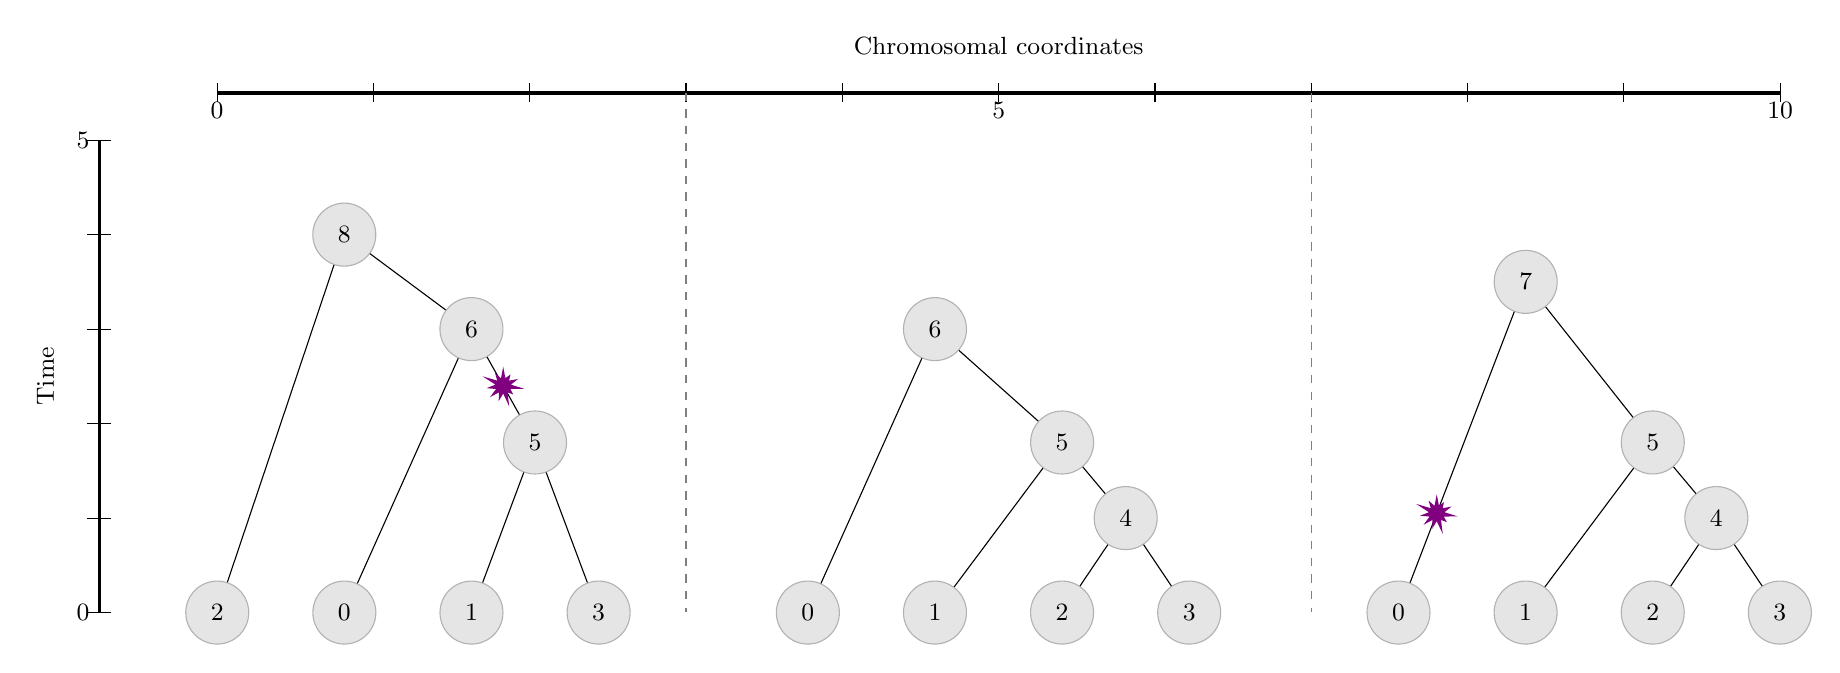
\begin{tikzpicture}[node distance=8mm and 8mm,xscale=1.5, yscale=1.2]

\tikzset{greynode/.style={font=\small,node distance=1cm and 1 cm,fill=black!10,draw=black!30,inner sep=0pt,minimum size=8mm,shape=circle},
mutations/.style={shape=starburst,fill=red!50!blue,inner sep=2pt,starburst points=11,starburst point height=.2cm}}

% Middle sample nodes
\node (s1) [greynode] {0};
\node (s2) [right=of s1,greynode] {1};
\node (s3) [right=of s2,greynode] {2};
\node (s4) [right=of s3,greynode] {3};

% Left sample nodes
\node (leftTree) at (-5, 0) {};
\node[greynode] (s3l) at ($(s1) + (leftTree)$) {2};
\node[greynode] (s1l) at ($(s2) + (leftTree)$) {0};
\node[greynode] (s2l) at ($(s3) + (leftTree)$) {1};
\node[greynode] (s4l) at ($(s4) + (leftTree)$) {3};

% Right sample nodes
\node (rightTree) at (5, 0) {};
\node [greynode] (s1r) at ($(s1) + (rightTree)$) {0};
\node [greynode] (s2r) at ($(s2) + (rightTree)$) {1};
\node [greynode] (s3r) at ($(s3) + (rightTree)$) {2};
\node [greynode] (s4r) at ($(s4) + (rightTree)$) {3};

% Non-sample nodes
\node [greynode] (s5) at ($0.5*(s3) + 0.5*(s4) + (0,1)$) {4};
\node [greynode] (s5r) at ($(s5) + (rightTree)$) {4};
\node [greynode] (s6) at ($(s3) + (0,1.8)$) {5};
\node [greynode] (s6r) at ($(s6) + (rightTree)$) {5};
\node [greynode] (s6l) at ($0.5*(s2l) + 0.5*(s4l) + (0,1.8)$) {5};
\node [greynode] (s7) at ($(s2) + (0,3)$) {6};
\node [greynode] (s7l) at ($(s2l) + (0,3)$) {6};
\node [greynode] (s8r) at ($(s2r) + (0,3.5)$) {7};
\node [greynode] (s9l) at ($(s1l) + (0,4)$) {8};

% Edges 
\draw (s6l) -- (s2l); \draw (s6l) -- (s4l); \draw (s7l) -- (s1l); \draw (s7l) -- (s6l); \draw (s3l) -- (s9l); \draw (s9l) -- (s7l); %tree 1
\draw (s5) -- (s3); \draw (s5) -- (s4); \draw (s6) -- (s2); \draw (s6) -- (s5); \draw (s7) -- (s1); \draw (s7) -- (s6); % tree 2
\draw (s5r) -- (s3r); \draw (s5r) -- (s4r); \draw (s6r) -- (s2r); \draw (s6r) -- (s5r); \draw (s8r) -- (s1r); \draw (s8r) -- (s6r); % tree 3

% Axes
\node (leftAx) at (-6,0) {};
\draw[very thick] (-6,0) -- +(0, 5);
\foreach \y in {0, 1, 2, 3, 4, 5} \draw ($(leftAx) + (-0.1, \y)$) -- ($(leftAx) + (0.1, \y)$); % tick marks
\draw[very thick] ($(s3l) + (0,5.5)$) -- ($(s4r) + (0,5.5)$);
\node (topAx) at (0,5.5) {};
\node (topLeft) at ($(s3l) + (0,5.5)$) {};
\node (genUnit) at ($0.1*(s4r) - 0.1*(s3l)$) {};
\foreach \x in {0, 1, 2, 3, 4, 5, 6, 7, 8, 9, 10} \draw ($(topLeft) + \x*(genUnit) + (0,0.1)$) -- +(0, -0.2); % tick marks
\node[anchor=east] at ($(leftAx)$) {\small 0}; \node[anchor=east] at ($(leftAx) + (0,5)$) {\small 5};
\node[anchor=north] at ($(topLeft)$) {\small 0}; \node[anchor=north] at ($(topLeft) + 5*(genUnit)$) {\small 5}; \node[anchor=north] at ($(topLeft) + 10*(genUnit)$) {\small 10};

% Interval endpoints
\draw[thin,color=black!50,dashed] ($(topLeft) + 3*(genUnit)$) -- +(0, -5.5);
\draw[thin,color=black!50,dashed] ($(topLeft) + 7*(genUnit)$) -- +(0, -5.5);

% Axis titles
\node (topLabel) at ($(topLeft) + 5*(genUnit) + (0,.5)$) {$\small\textrm{Chromosomal coordinates}$};
\node[rotate=90,anchor=south] (leftLabel) at ($(leftAx) + (-0.3,2.5)$) {$\small\textrm{Time}$};

% Mutations
\node [mutations] (m1) at ($(s6l)!.5!(s7l)$) {};
\node [mutations] (m1) at ($(s1r)!.3!(s8r)$) {};

\end{tikzpicture}

\[
\Updownarrow
\]
{\small
\renewcommand\baselinestretch{0.8}\selectfont
\begin{tabularx}{.05\textwidth}{p{1.5cm}X}
\toprule
\multicolumn{2}{c}{{\bf Nodes}}\\
\midrule
ID & time  \\
\midrule
0 & 0.0 \\
1 & 0.0\\
2 & 0.0\\
3 & 0.0\\
4 & 1.1\\
5 & 1.8\\
6 & 3.0\\
7 & 3.5\\
8 & 4.0\\
 & \\
 & \\
 \end{tabularx}\quad\quad\begin{tabularx}{.10\textwidth}{p{1.5cm}p{1.5cm}p{2cm}X}
\toprule
\multicolumn{4}{c}{{\bf Edges}}\\
\midrule
left & right & parent & child  \\
\midrule
3.0 & 10.0 & 4 & 2 \\
3.0 & 10.0 & 4 & 3\\
0.0 & 10.0 & 5 & 1\\
0.0 & 3.0 & 5 & 3\\
3.0 & 10.0 & 5 & 4\\
0.0 & 7.0 & 6 & 0\\
0.0 & 7.0 & 6 & 5 \\
7.0 & 10.0 & 7 & 0\\
7.0 & 10.0 & 7 & 5\\
0.0 & 3.0 & 8 & 2\\
0.0 & 3.0 & 8 & 6 \\
\end{tabularx}\quad\quad\begin{tabularx}{.08\textwidth}{p{2.5cm}p{1.5cm}X}
\toprule
\multicolumn{3}{c}{{\bf Mutations}}\\
\midrule
location & time& node  \\
\midrule
1.5 & 2.3 & 5\\
8.9 & 1.2 & 0\\
 & &\\
 & &\\
 & &\\
 & &\\
 & &\\
 & &\\
 & &\\
 & & \\
 & & \\
 \end{tabularx}
}
\end{center}
\vspace{10mm}
{\fontsize{35}{35}\selectfont
The \magenta{tree sequence} data structure [1,2] encodes a complete genealogy for a sample of chromosomes in a succinct set of tables. Compared with traditional sequence-based formats, tree sequences are \emph{compact}, \emph{fast} to process and \emph{informative} of the history of the sample.}
%Storing $n = 1\times 10^5$ chromosomes in a compressed VCF requires $\approx$ 50 GB.
%{\fontsize{35}{35}\selectfont However, common haplotypes in a sample are often simply a consequence of some common history. So if we know this history (as we always do in simulations!), storing it directly is often more convenient and efficient than storing the raw haplotypes. This is the key idea behind the \magenta{tree sequence} data structure [1,2], which encodes a complete genealogy for a sample of chromosomes in a succinct set of tables.\\
%Tree sequences offer a few benefits to population geneticists compared with traditional sequence-based file formats:
%
%\begin{itemize}
%\item They can store large simulated datasets extremely compactly.
%
%\item As they hold rich detail about the history of the sample, many important processes can be observed directly from the tree structure.
%
%\item They can be queried and modified extremely quickly.
%\end{itemize}}
     }
     
     %%%% BLOCK 3
     \block[titleoffsety=1cm,bodyoffsety=4cm]{3. Example: total IBD sharing over time}{
     } 
\centering
  \begin{subcolumns}
  \subcolumn{.6}
  \block{}{
  \centering
  

%% Set up the document
%\documentclass[convert={density=300,size=1080x800,outext=.png}]{standalone}
%
%% Include any extra LaTeX packages required
%%\usepackage[square, numbers, comma, sort&compress]{natbib}  % Use the "Natbib" style for the references in the Bibliography
%
%\usepackage{verbatim}  % Needed for the "comment" environment to make LaTeX comments
%\usepackage[table,x11names]{xcolor} % needed for highlighted rows
%
%\usepackage{tabularx,booktabs,adjustbox} % For tables
%\usepackage{pdflscape} % For writing some pages in landscape mode
%\usepackage{afterpage} % For control over the positioning of figures and tables.
%
%% For pictures
%\usepackage{tikz}
%\usetikzlibrary{calc,fit,arrows,decorations.pathmorphing,backgrounds,fit,positioning}
%\usetikzlibrary{shapes.symbols}
%
%% tikz colour settings
%\tikzset{pop0/.style={red!50!yellow},pop1/.style={violet!80},pop2/.style={olive!70!green}}
%
%%% ----------------------------------------------------------------
%\begin{document}
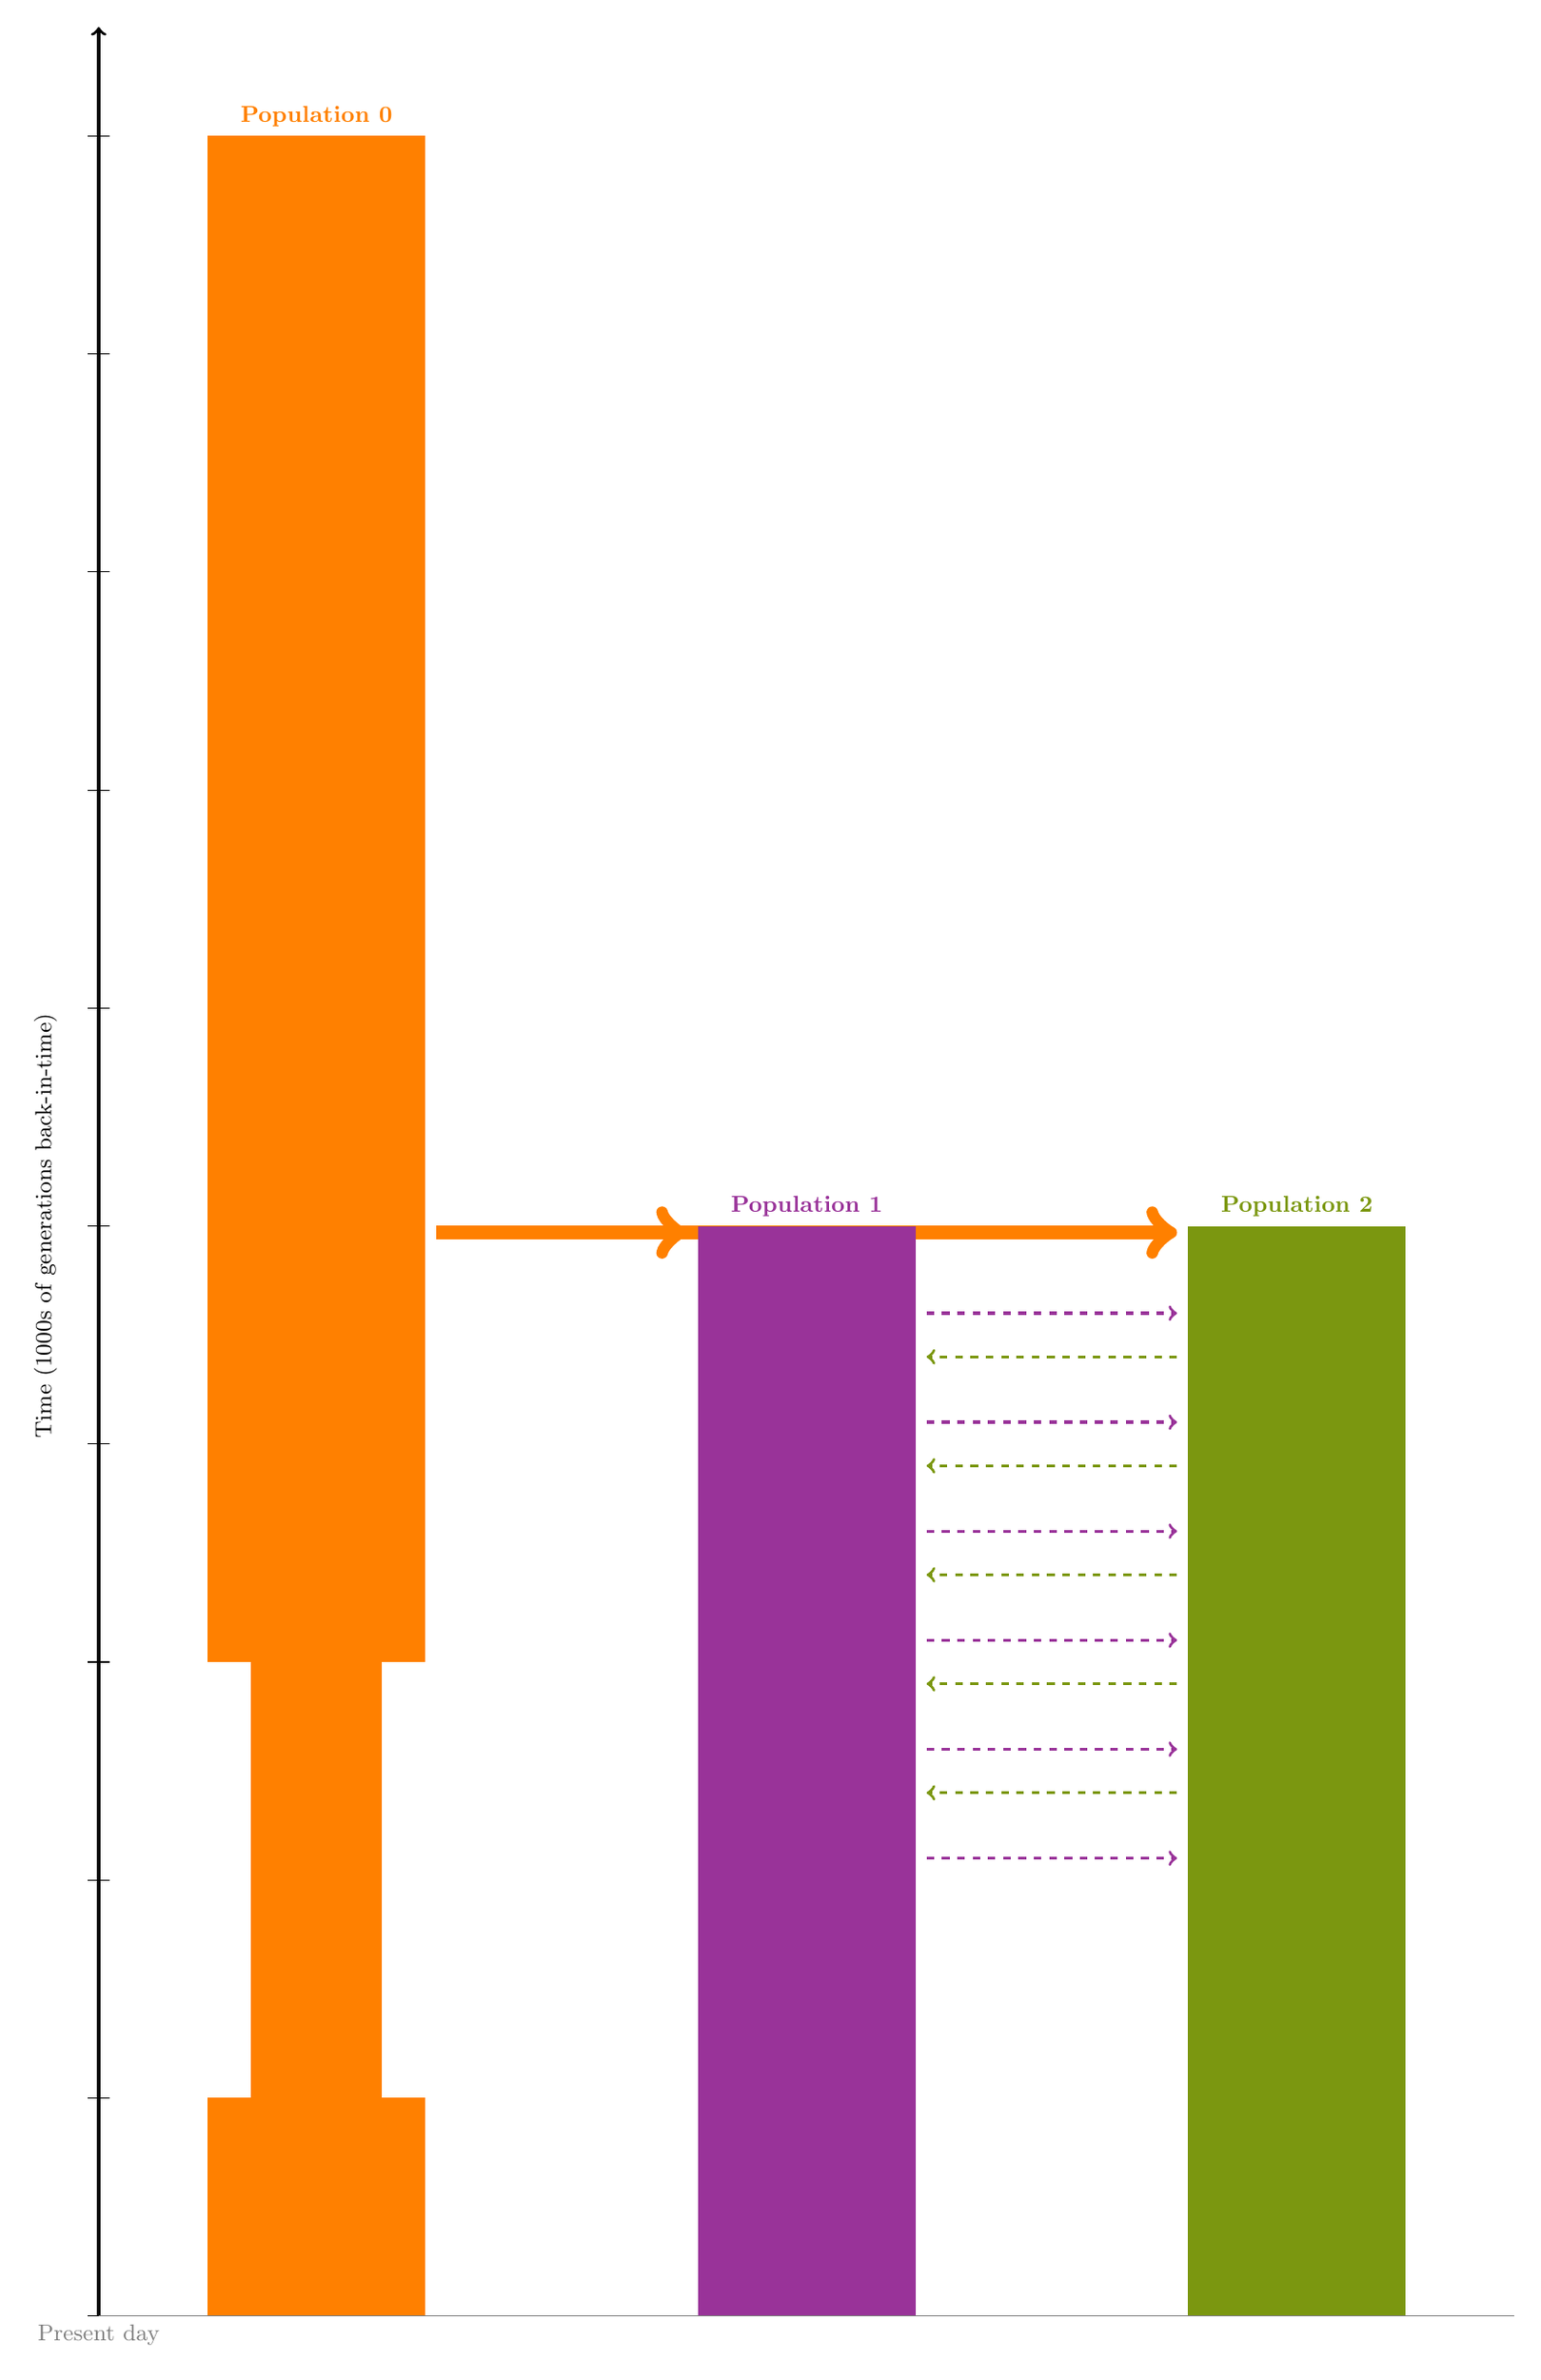
\begin{tikzpicture}[node distance=5mm and 5mm, xscale=1.5, yscale=3]

\tikzset{greynode/.style={font=\footnotesize,node distance=1cm and 1 cm,fill=black!10,draw=black!30,inner sep=0pt,minimum size=3.5mm,shape=circle},
mutations/.style={shape=starburst,fill=red!50!blue,inner sep=0.8pt,starburst points=11,starburst point height=.2cm}}

% Nodes
\node (origin) at (0,0){};
\node (pop0) at (1,0){};
\node (pop1) at (5.5,0){};
\node (pop2) at (10,0){};
\node (popwidth) at (2,0){};

% Axis
\node (leftAx) at (-1,0) {};
\draw[very thick,->] (-1,0) -- +(0, 10.5);
\foreach \y in {0, 1, 2, 3, 4, 5, 6, 7, 8, 9, 10} \draw ($(leftAx) + (-0.1, \y)$) -- ($(leftAx) + (0.1, \y)$); % tick marks
%\node[anchor=east] at ($(leftAx)$) {0}; \node[anchor=east] at ($(leftAx) + (0,5)$) {5};
\node[rotate=90,anchor=south] (leftLabel) at ($(leftAx) + (-0.3,5)$) {\small$\textrm{Time (1000s of generations back-in-time)}$};

% Migrations
\foreach \y in {1.5,2,2.5,3,3.5,4} \draw[pop1,dashed,->,very thick] ($(.1,.1) + (leftAx) + (0,\y + .5)+(pop1) + (popwidth)$) -- +(2.3,0);
\foreach \y in {2,2.5,3,3.5,4} \draw[pop2,dashed,->,very thick] ($(-.1,-.1) + (leftAx) + (0,\y + .5)+(pop2)$) -- +(-2.3,0);
\draw[pop0, ->, line width=2mm] ($(.1,0) + (leftAx) + (0,4.97)+(pop0) + (popwidth)$) -- +(2.3,0);
\draw[pop0, ->, line width=2mm] ($(.1,0) + (leftAx) + (0,4.97)+(pop0) + 2*(popwidth)$) -- +($2*(2.4,0)$);

% Populations
\foreach \x in {0} \fill[pop\x] ($(leftAx) + (pop\x)$) -- ++(0,10) -- ++(2, 0) -- ++(0, -10) -- cycle;
\foreach \x in {1, 2} \fill[pop\x] ($(leftAx) + (pop\x)$) -- ++(0,5) -- ++(2, 0) -- ++(0, -5) -- cycle;
\foreach \x in {0} \node[above,pop\x] (label\x) at ($(leftAx) + (pop\x) + (1, 10)$) {\small\bf Population \x};
\foreach \x in {1,2} \node[above,pop\x] (label\x) at ($(leftAx) + (pop\x) + (1, 5)$) {\small\bf Population \x};

% Times
\draw[very thin,color=gray] (-1,0) node[below] {\small Present day} -- (12,0);

% White squares over pop0 bottleneck areas.
\fill[white] ($(leftAx) + 0.9*(pop0) + (0,1)$) -- ++($0.5*(pop0)$) -- ++(0,2) -- ++($-0.5*(pop0)$) -- cycle;
\fill[white] ($(leftAx) + 1.1*(pop0) +(popwidth) + (0,1)$) -- ++($-0.5*(pop0)$) -- ++(0,2) -- ++($0.5*(pop0)$) -- cycle;

% Grey dashed arrows
%\foreach \y in {2,4,6,8,10} \draw[gray,densely dashed,->] ($(12,\y)$) -- +(4,0);

\end{tikzpicture} 
%\end{document}  % The End
%%% ----------------------------------------------------------------
%  \input{pics/new-method/simulation-method-0.tex}
%    \input{pics/new-method/simulation-method-2.tex}
%      \input{pics/new-method/simulation-method-4.tex}
  }
  \subcolumn{.35}
   \block{}{
   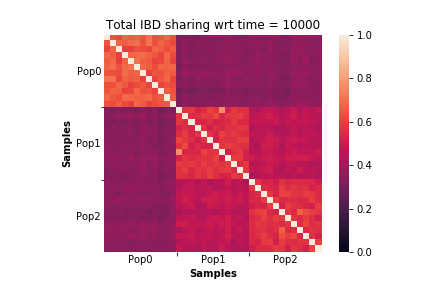
\includegraphics[scale=.63]{pics/kinships-10000.png}
   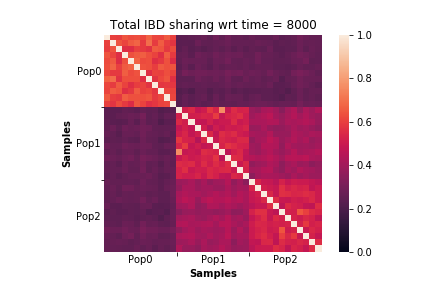
\includegraphics[scale=.63]{pics/kinships-8000.png}
    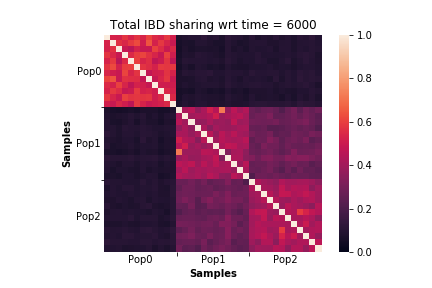
\includegraphics[scale=.63]{pics/kinships-6000.png}
    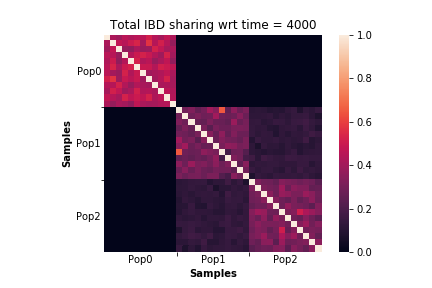
\includegraphics[scale=.63]{pics/kinships-4000.png}
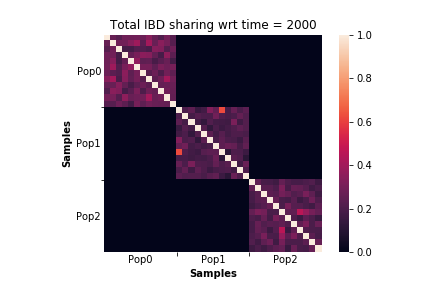
\includegraphics[scale=.63]{pics/kinships-2000.png}

  }
  \end{subcolumns}



     \column{.5}
     %%% BLOCK 2
         \block[titleoffsety=-3cm,bodyoffsety=1.5cm]{2. IBD and ancestry in tree sequences}{}  
%          \begin{subcolumns}       
%         \subcolumn{.45}
          \block{}{
          \begin{center}
          \begin{center}
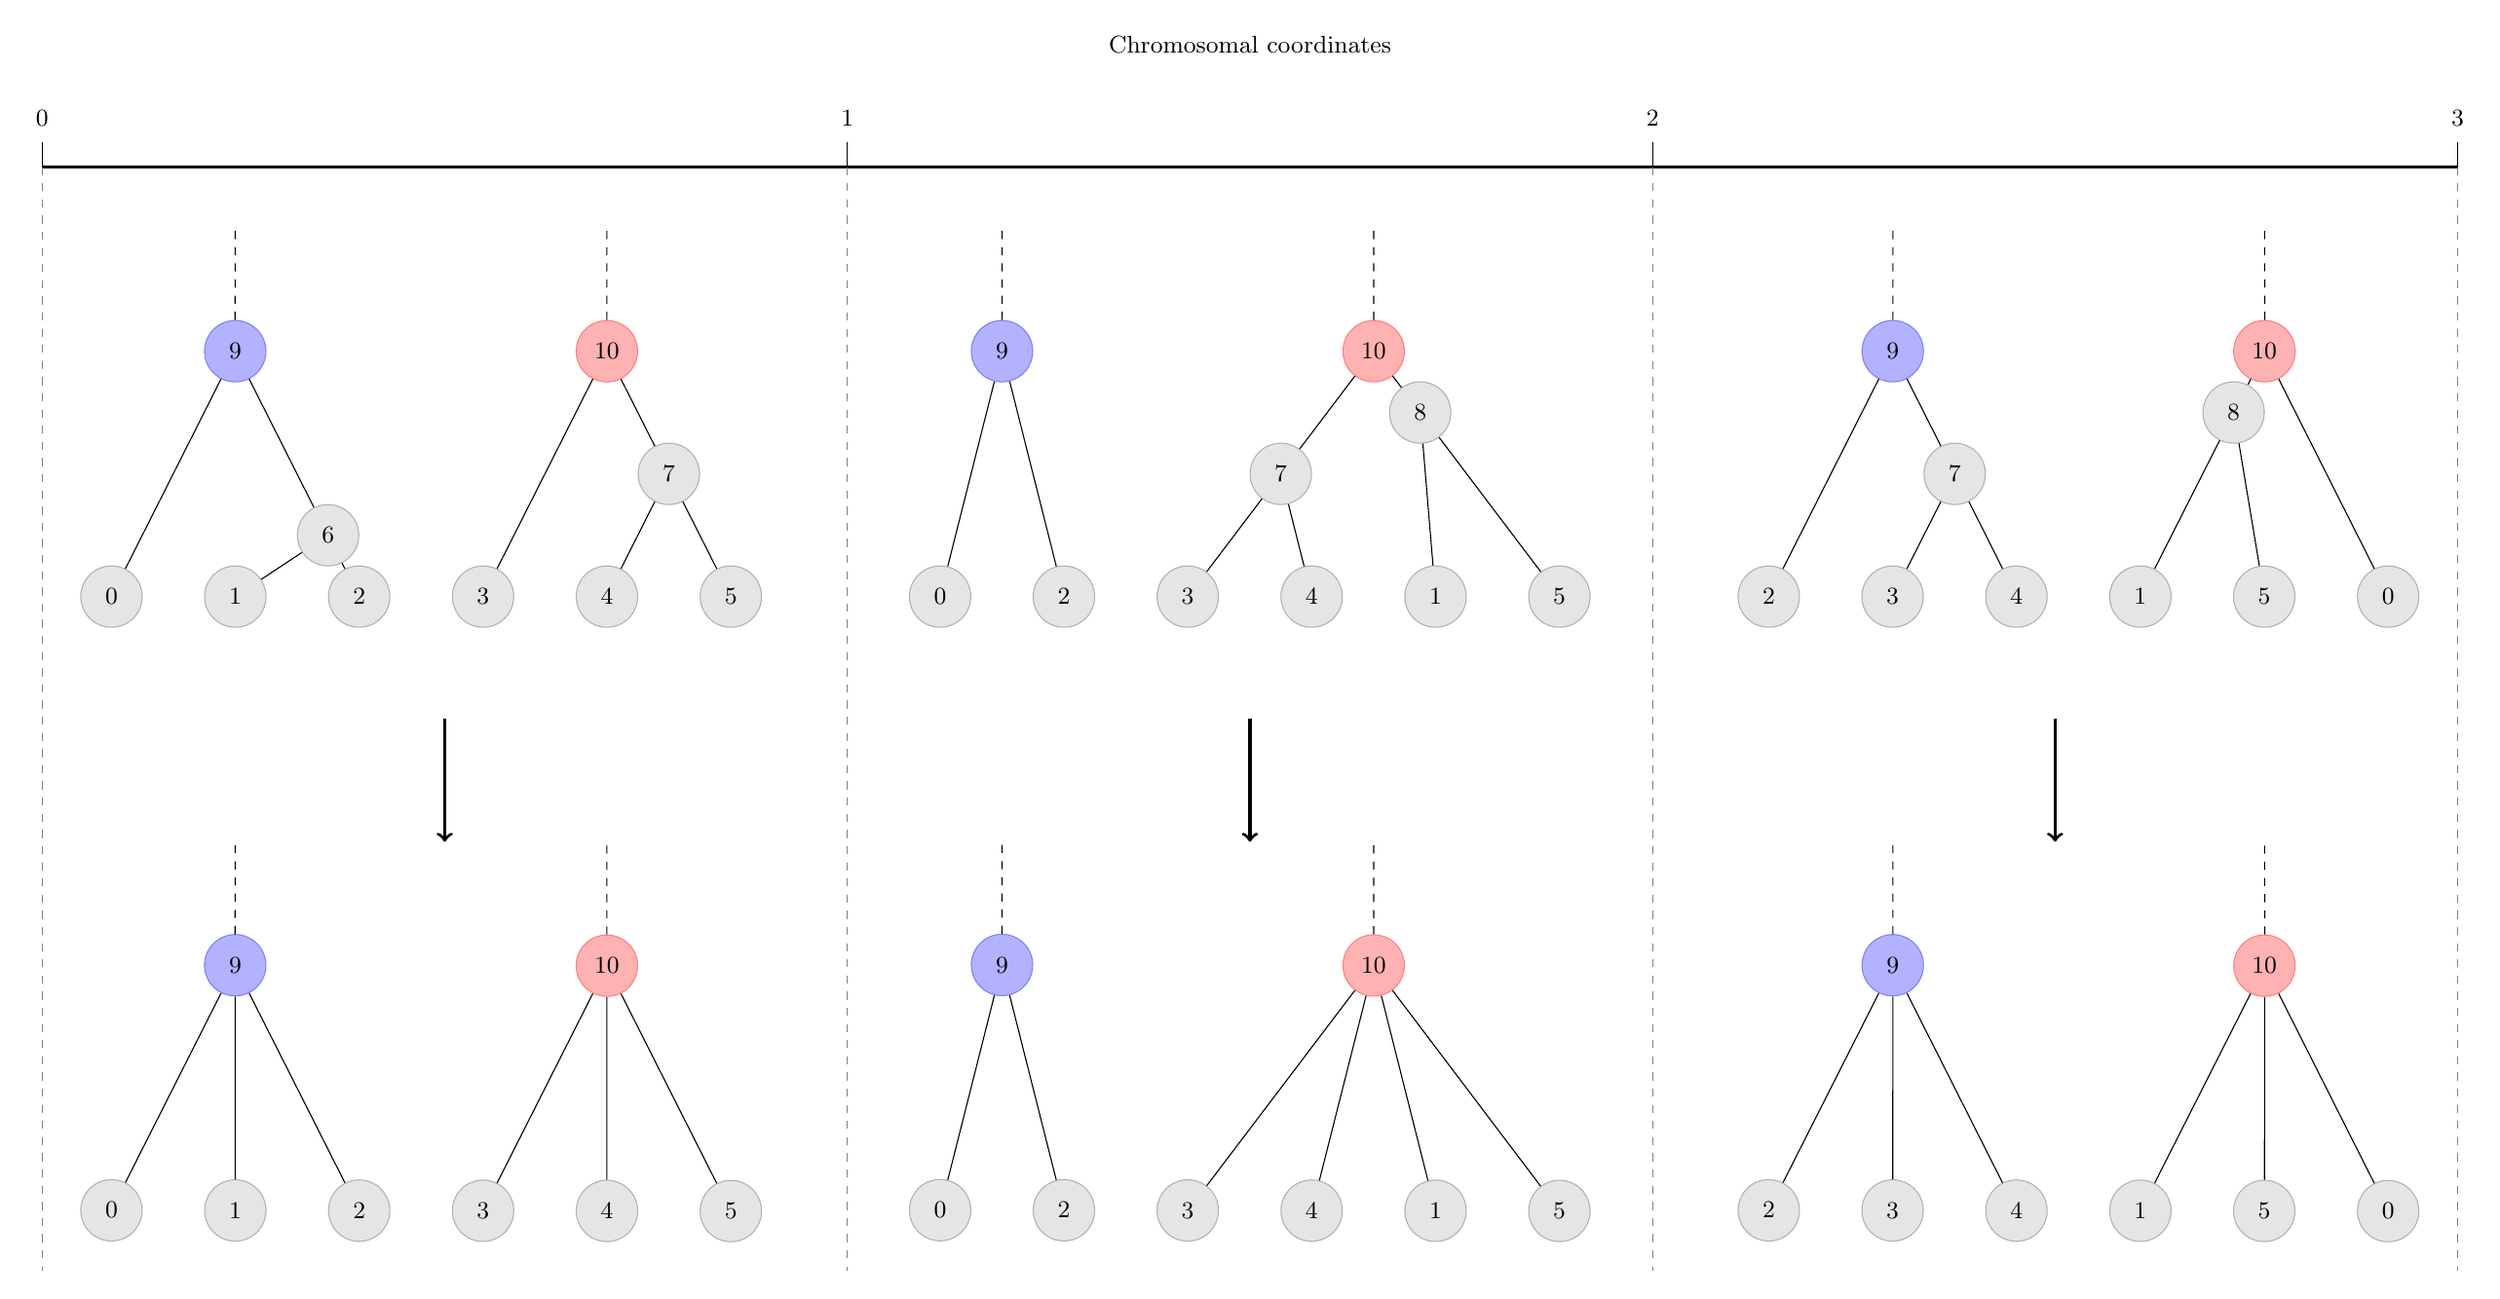
\begin{tikzpicture}[node distance=8mm and 8mm,xscale=1.8,yscale=1.6]

\tikzset{greynode/.style={font=\small,node distance=.5cm and .5 cm,fill=black!10,draw=black!30,inner sep=0pt,minimum size=8mm,shape=circle},
bluenode/.style={font=\small,node distance=.5cm and .5cm,fill=blue!30,draw=blue!50,inner sep=0pt,minimum size=8mm,shape=circle},
rednode/.style={font=\small,node distance=.5cm and .5cm,fill=red!30,draw=red!50,inner sep=0pt,minimum size=8mm,shape=circle}}

% Middle sample nodes
\node (s0) [greynode] {0};
\node (s2) [right=of s0,greynode] {2};
\node (s3) [right=of s2,greynode] {3};
\node (s4) [right=of s3,greynode] {4};
\node (s1) [right=of s4,greynode] {1};
\node (s5) [right=of s1,greynode] {5};

% Left sample nodes
\node (leftTree) at (-6, 0) {};
\node[greynode] (s0l) at ($(s0) + (leftTree)$) {0};
\node[greynode] (s1l) at ($(s2) + (leftTree)$) {1};
\node[greynode] (s2l) at ($(s3) + (leftTree)$) {2};
\node[greynode] (s3l) at ($(s4) + (leftTree)$) {3};
\node[greynode] (s4l) at ($(s1) + (leftTree)$) {4};
\node[greynode] (s5l) at ($(s5) + (leftTree)$) {5};

% Right sample nodes
\node (rightTree) at (6, 0) {};
\node [greynode] (s2r) at ($(s0) + (rightTree)$) {2};
\node [greynode] (s3r) at ($(s2) + (rightTree)$) {3};
\node [greynode] (s4r) at ($(s3) + (rightTree)$) {4};
\node [greynode] (s1r) at ($(s4) + (rightTree)$) {1};
\node [greynode] (s5r) at ($(s1) + (rightTree)$) {5};
\node [greynode] (s0r) at ($(s5) + (rightTree)$) {0};

% Ancestral nodes
\node (anc) at (0,2) {};
\node[bluenode] (s9) at ($0.5*(s0) + 0.5*(s2) + (anc)$) {9};
\node[bluenode] (s9l) at ($0.5*(s0l) + 0.5*(s2l) + (anc)$) {9};
\node[bluenode] (s9r) at ($0.5*(s2r) + 0.5*(s4r) + (anc)$) {9};
\node[rednode] (s10) at ($0.5*(s3)+0.5*(s5) + (anc)$) {10};
\node[rednode] (s10l) at ($0.5*(s3l)+0.5*(s5l) + (anc)$) {10};
\node[rednode] (s10r) at ($0.5*(s1r)+0.5*(s0r) + (anc)$) {10};

% Internal nodes
\node[greynode] (s6l) at ($(s2l)!0.25!(s9l)$) {6};
\node[greynode] (s7) at ($(s3)!.5!(s10)$) {7};
\node[greynode] (s7l) at ($(s5l)!.5!(s10l)$) {7};
\node[greynode] (s7r) at ($(s4r)!.5!(s9r)$) {7};
\node[greynode] (s8) at ($(s5)!.75!(s10)$) {8};
\node[greynode] (s8r) at ($(s1r)!.75!(s10r)$) {8};

% Edges
\draw (s0) -- (s9) -- (s2); \draw (s3) -- (s7) -- (s10) -- (s8) -- (s5); \draw (s4) -- (s7); \draw (s1) -- (s8); % middle tree
\draw (s0l) -- (s9l) -- (s6l) -- (s2l); \draw (s1l) -- (s6l); \draw ( s3l) -- (s10l) -- (s7l) -- (s5l); \draw (s4l) -- (s7l); % left tree
\draw (s2r) -- (s9r) -- (s7r) -- (s4r); \draw (s3r) -- (s7r); \draw (s1r) -- (s8r) -- (s10r) -- (s0r); \draw (s5r) -- (s8r); % right tree
\draw[dashed] (s9) -- +(0,1); \draw[dashed] (s9l) -- +(0,1); \draw[dashed] (s9r) -- +(0,1);
\draw[dashed] (s10) -- +(0,1); \draw[dashed] (s10l) -- +(0,1); \draw[dashed] (s10r) -- +(0,1);

% Axes
\node (topAx) at (0,3.5) {};
\node (topLeft) at ($(s0l) + (topAx) + (-0.5, 0)$) {};
\node (topRight) at ($(s0r) + (topAx) + (0.5,0)$) {};
\draw[very thick] (topLeft.center) -- (topRight.center);
\node (genunit) at ($0.3333*(topRight) - 0.3333*(topLeft)$) {};
\foreach \x in {0,1,2,3} \draw ($(topLeft) + \x*(genunit)$) -- +(0,.2);
\foreach \x in {0,1,2,3} \node at ($(topLeft) + \x*(genunit) + (0,.4)$) {\small\x};

% Interval endpoints
\foreach \x in {0,1,2,3} \draw[thin,color=black!50,dashed] ($(topLeft) + \x*(genunit)$) -- +(0, -9);
%\draw[thin,color=black!50,dashed] ($(topLeft) + 7*(genUnit)$) -- +(0, -5.5);

% Axis titles
\node (topLabel) at ($(topLeft) + 1.5*(genunit) + (0,1)$) {\small$\textrm{Chromosomal coordinates}$};

%%%%%
\node (after) at (0, -5) {};

% Middle sample nodes
\node[greynode] (s0) at (after) {0};
\node (s2) [right=of s0,greynode] {2};
\node (s3) [right=of s2,greynode] {3};
\node (s4) [right=of s3,greynode] {4};
\node (s1) [right=of s4,greynode] {1};
\node (s5) [right=of s1,greynode] {5};

% Left sample nodes
\node (leftTree) at (-6, 0) {};
\node[greynode] (s0l) at ($(s0) + (leftTree)$) {0};
\node[greynode] (s1l) at ($(s2) + (leftTree)$) {1};
\node[greynode] (s2l) at ($(s3) + (leftTree)$) {2};
\node[greynode] (s3l) at ($(s4) + (leftTree)$) {3};
\node[greynode] (s4l) at ($(s1) + (leftTree)$) {4};
\node[greynode] (s5l) at ($(s5) + (leftTree)$) {5};

% Right sample nodes
\node (rightTree) at (6, 0) {};
\node [greynode] (s2r) at ($(s0) + (rightTree)$) {2};
\node [greynode] (s3r) at ($(s2) + (rightTree)$) {3};
\node [greynode] (s4r) at ($(s3) + (rightTree)$) {4};
\node [greynode] (s1r) at ($(s4) + (rightTree)$) {1};
\node [greynode] (s5r) at ($(s1) + (rightTree)$) {5};
\node [greynode] (s0r) at ($(s5) + (rightTree)$) {0};

% Ancestral nodes
\node (anc) at (0,2) {};
\node[bluenode] (s9) at ($0.5*(s0) + 0.5*(s2) + (anc)$) {9};
\node[bluenode] (s9l) at ($0.5*(s0l) + 0.5*(s2l) + (anc)$) {9};
\node[bluenode] (s9r) at ($0.5*(s2r) + 0.5*(s4r) + (anc)$) {9};
\node[rednode] (s10) at ($0.5*(s3)+0.5*(s5) + (anc)$) {10};
\node[rednode] (s10l) at ($0.5*(s3l)+0.5*(s5l) + (anc)$) {10};
\node[rednode] (s10r) at ($0.5*(s1r)+0.5*(s0r) + (anc)$) {10};

%% Axes
%\node (topAx) at (0,3.5) {};
%\node (topLeft) at ($(s0l) + (topAx) + (-0.5, 0)$) {};
%\node (topRight) at ($(s0r) + (topAx) + (0.5,0)$) {};
%\draw[very thick] (topLeft.center) -- (topRight.center);
%\node (genunit) at ($0.3333*(topRight) - 0.3333*(topLeft)$) {};
%\foreach \x in {0,1,2,3} \draw ($(topLeft) + \x*(genunit)$) -- +(0,.2);
%\foreach \x in {0,1,2,3} \node at ($(topLeft) + \x*(genunit) + (0,.4)$) {\x};

% Edges
\draw (s0) -- (s9) -- (s2); \draw (s3) -- (s10) -- (s4); \draw (s1) -- (s10) --  (s5); % middle tree
\draw (s0l) -- (s9l) -- (s2l); \draw (s1l) -- (s9l); \draw (s3l) -- (s10l) -- (s5l); \draw (s4l) -- (s10l); % left tree
\draw (s2r) -- (s9r) -- (s3r); \draw (s4r) -- (s9r); \draw (s1r) -- (s10r) -- (s5r); \draw (s0r) -- (s10r);

\draw[dashed] (s9) -- +(0,1); \draw[dashed] (s9l) -- +(0,1); \draw[dashed] (s9r) -- +(0,1);
\draw[dashed] (s10) -- +(0,1); \draw[dashed] (s10l) -- +(0,1); \draw[dashed] (s10r) -- +(0,1);

% Interval endpoints
\foreach \x in {0,1,2,3} \draw[thin,color=black!50,dashed] ($(topLeft) + \x*(genunit)$) -- +(0, -4);
%\draw[thin,color=black!50,dashed] ($(topLeft) + 7*(genUnit)$) -- +(0, -5.5);

%% Axis titles
%\node (topLabel) at ($(topLeft) + 1.5*(genunit) + (0,1)$) {$\textrm{Chromosomal coordinates}$};

%% Arrows
\foreach \x in {0, 1, 2} \draw[<-,very thick] ($(topLeft) + \x*(genunit) + 0.5*(genunit) + (0,-5.5)$) -- +(0, 1);

\end{tikzpicture}
\end{center} 
          \end{center}
{\fontsize{34}{35}\selectfont Questions about inheritance and ancestry can be reframed as questions about the underlying tree sequence that represents the data:
          \begin{itemize}
          \item {\it \magenta{Identity-by-descent}: which samples share a common ancestor? How recently? Over which genomic interval?}
          \item {\it \magenta{Local ancestry}: which ancestors have which population labels? Which samples descend from them? Over which genomic interval?}
          \end{itemize}
Extracting this information from large datasets requires efficient algorithms that account for the correlations in genealogical structure between samples, and across chromosomes.}
          }           
       
\vspace{20cm}

             \block[titleoffsety=0cm,bodyoffsety=0cm]{4. Application: demography inference}{
{\fontsize{34}{35}\selectfont To explore the power of our method, we attempted to recreate some of the important findings from a recent study of Ashkenazi Jewish (AJ) demographic history [3]. This work provided evidence for a recent divergence event between Eastern and Western communities of AJ people. It was estimated that this happened about 15 generations ago.\\[2mm]
Closely following [3], we performed 50 000 simulations of various demographic scenarios. For each simulation, we calculated moments of IBD segment lengths at multiple time points. We used the \texttt{abcrf} package [4] to infer the most plausible demographic scenario, and the \texttt{abc} package [5] with neural-net regression to estimate parameter values.\\

{\bf Results: inference of demographic scenario}
\begin{center}
\begin{tabularx}{.45\textwidth}{p{11cm}p{15cm}X}
\toprule
Posterior probability & Votes for correct scenario & Prior error rate \\
\midrule
$93.36\% \pm 4.69\%$ &	$0.9633 \pm 0.0268$	& $0.0993 \pm 0.0008$\\
\bottomrule\\
\end{tabularx}
\end{center}

{\bf Results: inference of divergence time}
\begin{center}
\begin{tabularx}{.45\textwidth}{p{5cm}p{7cm}p{10cm}X}
\toprule
Mode & True value & Our 95\% HPDI & 95\% HPDI in [3] \\
\midrule
13.59 & 14.93 & $(11.22, 19.90)$ & $(2.00, 29.00)$\\
\bottomrule\\
\end{tabularx}
\end{center}
All simulations and analyses ran on a standard desktop in $<12$ hours.}
}
     \end{columns}

%%% BLOCK 5
 \block[titleoffsety=1cm,bodyoffsety=1cm]{5. Acknowledgements, references and further information}{
 }
  \begin{columns}
 \begin{subcolumns}
    \subcolumn{22} \block[bodyoffsetx=1.5cm,bodyverticalshift=-5cm]{}{\footnotesize
     GT is funded by the Helen Freeman scholarship, the Maurice Belz Fund and the Australian Government's Research Training Scheme.\\[1mm]
     [1] \texttt{https://tskit.readthedocs.io/en/latest/}\\[1mm]
     [2] Kelleher, J., et al. (2016). Efficient Coalescent Simulation and Genealogical Analysis for Large Sample Sizes. PLOS Computational Biology, 12(5).\\[1mm]
     [3] Gladstein, A and Hammer, M. (2019). Substructured Population Growth in the Ashkenazi Jews Inferred with Approximate Bayesian Computation. Molecular Biology and Evolution, 36(6), 1162-1171.\\[1mm] 
    [4] Raynal, L., et al. (2019). ABC random forests for Bayesian parameter inference. Bioinformatics, 35(10), 1720 - 1728.\\[1mm]
	[5] Csillery, K., et al. (2012). Abc: An R package for approximate Bayesian computation (ABC). Methods in Ecology and Evolution, 3(3), 475 - 479.
     }
       \subcolumn{3} \block[bodyoffsetx=-2cm,bodyverticalshift=-6cm]{}{
       \begin{center}
       
\includegraphics[scale=1]{pics/tskit-logo.png}
      \end{center}
       }
       \subcolumn{3} \block[bodyoffsetx=-1cm,bodyverticalshift=-5cm]{}{
       \begin{center}
       
\includegraphics[scale=1.2]{pics/unimelb-logo.jpg}
      \end{center}
       }
      \subcolumn{3} \block[bodyoffsetx=-3cm,bodyverticalshift=-5.7cm]{}{
       \begin{center}
       {\small Come say hi!}\\
       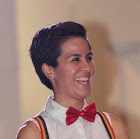
\includegraphics[scale=1]{pics/GT_headshot.jpg} 
       \end{center}
       }
 \end{subcolumns}
 \end{columns}         

 \end{document}




\endinput
%%
%% End of file `tikzposter-example.tex'.
